\section{Results}
The results of my work have two facets. The first being the degree that the system as it is currently implemented can classify phrases as Puns, and the second being the output of a framework that can be leveraged in future work and applying a new type of analysis to this problem. As I had stated in midterm  paper, the goal of the project wasn't to make the best classifier possible, but to explore this graph data structure and to see how some simple heuristics fit into it.

\subsection{Qualitiative Results}
One of the important accomplishments made was enabling the visualization of these pun graphs. By combining D3.js and the Graffeine project \cite{graffeine}, I was able to add a presentation layer above the Neo4J database that held the output graph of the heuristics applied by the analysis program. In Figure \ref{pungraphscreenshot}, a screenshot of the console can be seen. Another important capability of this graphical console is the ability to edit the nodes and edges of the graph. This would enable researchers and heuristic developers to manually edit and tweak the state of the graph to see how it affects their algorithms.

Because Neo4J can scale to handle large graphs, as the amount of analysis increases with more heuristics, the technique should scale with smart heuristic implementation. What is meant by smart implementation, is that heuristics leverage the query language of Neo4J to return only a subset of nodes and edges to process, instead of having to process the entire graph. This would not be easily possible for graphs that would be required to be held in-memory, as they could potentially exceed the working space of a machine, and don't have a rich built in query language.

\begin{center}
\begin{figure}[h]
  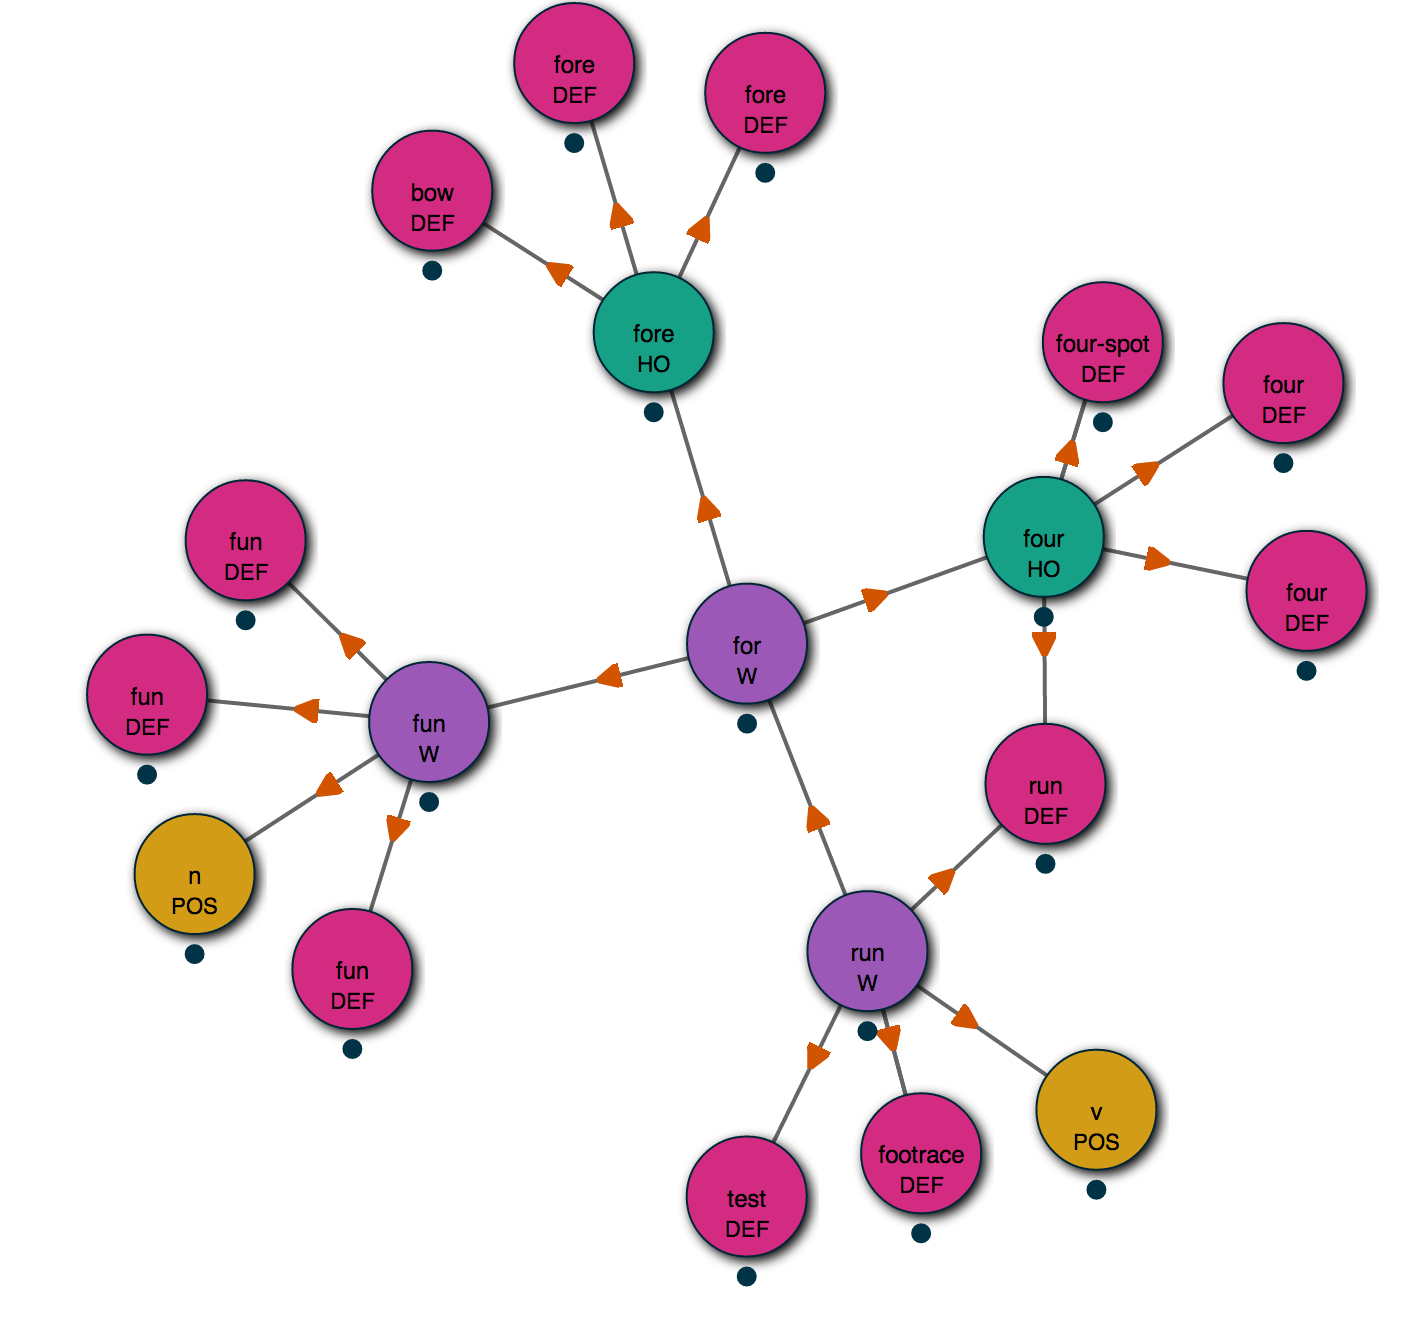
\includegraphics[keepaspectratio=true, scale=.35]{pun-graph.png}
  \caption{Screenshot of Puntective Implementation}
   \label{pungraphscreenshot}
\end{figure}
\end{center}

\subsection{Quantitative Results}
In an attempt to quantify the results my current implementation obtained I ran the set of heuristics against my dataset, and averaged the scores across both positive and negative examples. For the purpose of this test, I assigned the value of a 'definition linkage' as 10 points, and the presence of a homophone is worth 5 points.  We can see from the table of aggregate results that the heuristics I implemented are not quite enough to determine if something is a pun or not. This is due in part to their simplicity, and lack of depth. Going back to a qualitative approach for a moment, In some examples I tested, the `definition-linkage' heuristic did connect words in the graph together that showed humor connections (if a human were building a graph for the same phrase).

\begin{center}
'funniness score' for pun and non-pun examples.
 \begin{tabular}{||c c c c c||}
 \hline
 Type of Phrase & Average & Median & Max  & Min \\ [0.5ex] 
 \hline\hline
 Pun & 80.3 & 65.0 &  185 & 15 \\ 
 \hline
 Non-Pun & 135.0 & 105.0 & 515 & 0 \\
 \hline
\end{tabular}
\end{center}

In this case, I didn't attempt to determine where the `threshold' for the ascension from normal phrase to pun, since the techniques are still very unrefined, and the dataset is not large enough to be a representative sample of many kinds of phrases.

See Appendix A for detailed results.
